\section{Version 0.1}
The first version of this project included learning about the \gls{LSU} methodology and development of the application. It produced three movies in two iterations where the first movie included several user stories and the other two movies each represented a selected user story. The duration of this version was almost four weeks, but it included a lot of the ground work needed for the team to be able to develop an application and follow the lean startup methodology.

\subsection{Assumption}
The goal of this release was making a video explaining what the team assumed the purpose of the product would be. This was done to conduct a so called smoke test where the video was created to learn if it was enough users interested in the product.

\subsection{Planning and design}
After the first meeting where the team had been introduced to the customer and the idea of the product all the members  had to draw a sketch of what they thought the application would function. There had been some differences in the perception of the functionality, but at the second team meeting the different sketches were discussed and the team agreed upon what was thought to be the most important features of the application. 

With these features as a basis the initial \gls{mockup} of the application was created. It was decided that the most resource efficient manner of doing a smoke test was to make a simple video explaining the product. The \gls{mockup} was used to represent the potential application in the first demonstration movie. 

The team decided to gather the feedback from the movie using a survey on the website, and unstructured interviews. In the survey, users could add their email address in order to receive updates and become beta testers. 


From the feedback received of the first movie, the team learned that three different examples of use in one movie could seem confusing for the people who had never heard of the product. Due to this response, the team reconsidered the movie and decided decided that the users were likely to be students and companies. Based on this decision two new movies was created. Each represented one of these scenarios of use. These target groups were also available for contact through Netlight and fellow students. The two new movies were released on the same web page with an updated version of the feedback survey. 

In parallel with making the demonstration videos, it was agreed that the mobile teams should start creating the basis for the applications, and that the backend should start building the initial \gls{API} and consider different database options.


\subsection{Development}
An information video was the main focus during this first version, but in order to avoid spending unnecessary resources, the development on both client platforms and the backend was initiated.

\subsubsection{First demonstration movie} 
The first video was made using Balsamiq \cite{balsamiq} where the touches in the application was represented by a pointer. The movie told three stories to present possible use of the application while showing the functionality. The voice was recorded using Audacity. 

The first scenario in the movie was a woman named Jane who work at a company with a lot of books for collective use. It was then presented how the company could keep track of all these books using the new application.

The second scenario was Joseph who owns a lot of books. He likes to share them with his friends and can now, with the help of the application always have an overview of who has which book. 

The third scenario was Emma the student who is in a colloquium where the students like to share the course litterature among each other. In this scenario the crowd functionality is represented to show how she can see which books the colloquium has to offer.

The movie can be watch at \url{https://www.youtube.com/watch?v=7KbctbCdvvU} and a snapshot is shown in figure \ref{fig:information-film-01}.
\begin{figure}
\centering
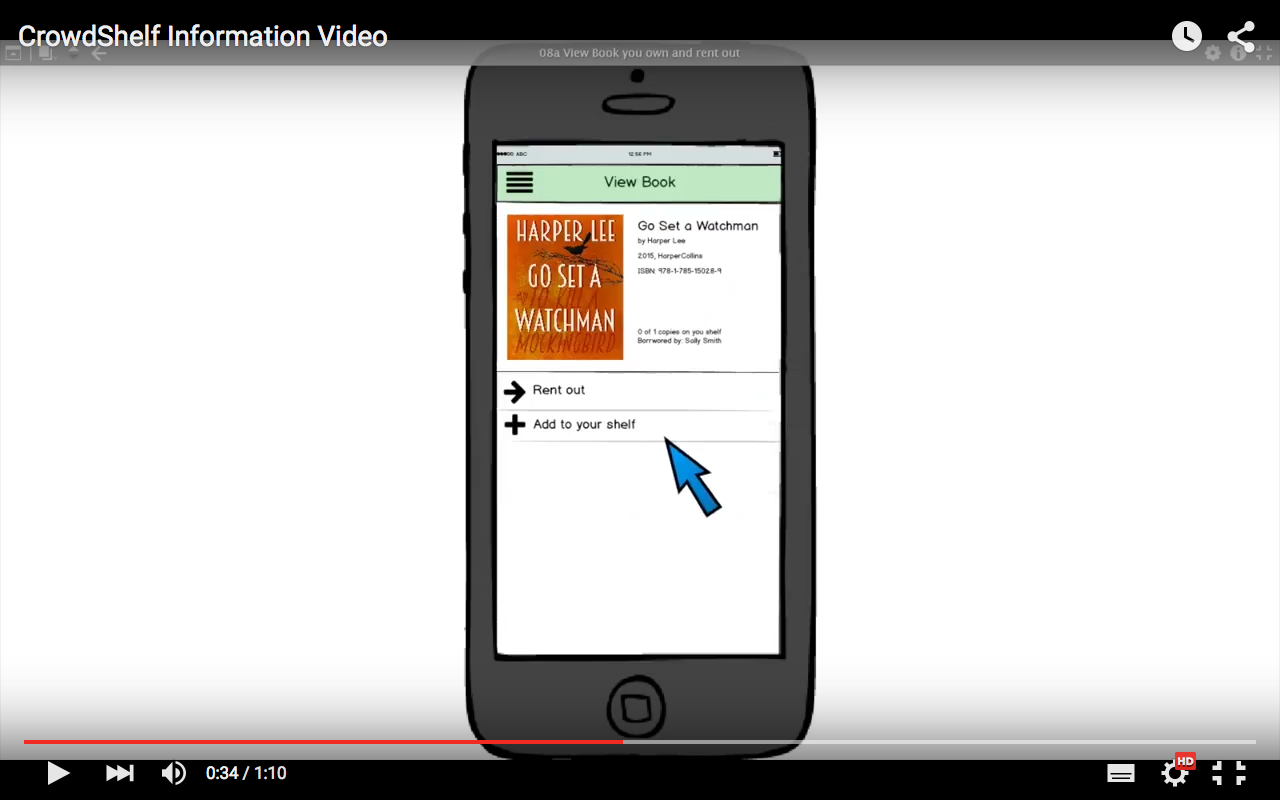
\includegraphics[height=5cm]{figs/v01/FirstInformationMovieBook.png}
\caption{Shot from the first demonstration movie}
\label{fig:information-film-01}
\end{figure}

\subsubsection{The student and company movies} 
The two movies that represented the student and company example respectively was created using Adobe Edge Animate to achieve a more professional look. 

The movie that represent the student example brought up the issue of buying expensive new books and that it is preferable maybe to borrow the books from fellow students. It then shows the students creating a crowd and adding other members. Afterwards the movie shows that the student finds out who has the desired book using the application and then seeks her out, scan the book with the application and borrow it. 

In the company example movie the focus is on the value of the employees competence and how that knowledge often is obtained by reading books. The problem occurs when the company’s shelf becomes empty and the employees can not find the books.The movie then shows how the company can create a crowd so that they and the employees can know where the books are at all times.

The videos were shared on Youtube and on the project's web site. They can be watched at \url{https://www.youtube.com/watch?v=yj0NNimKgIw} and \url{https://www.youtube.com/watch?v=6Nedobb4eZ0}. Snapshots from the movies are in figure \ref{fig:student-example} and figure \ref{fig:company-example}
\begin{figure}
\centering
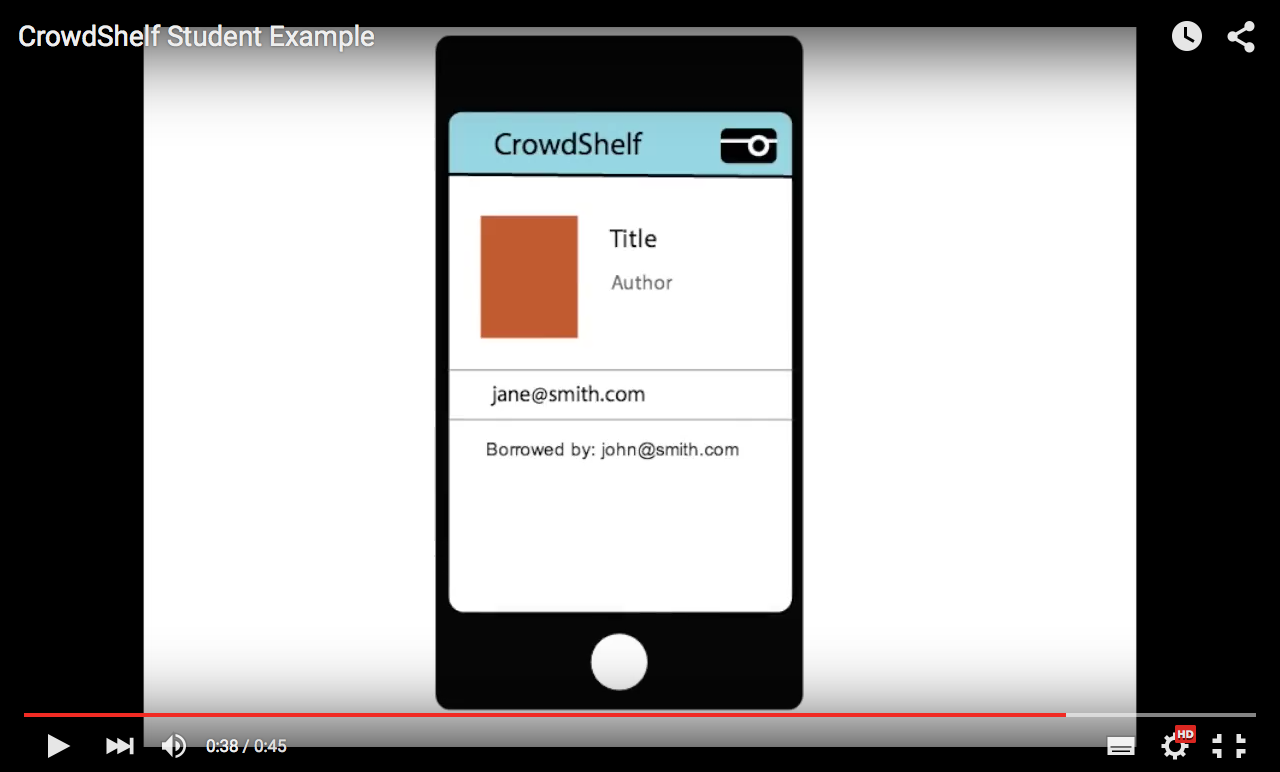
\includegraphics[height=5cm]{figs/v01/InfoMovieStudent2.png}
\caption{Shot from the student example demonstration movie}
\label{fig:student-example}
\end{figure}

\begin{figure}
\centering
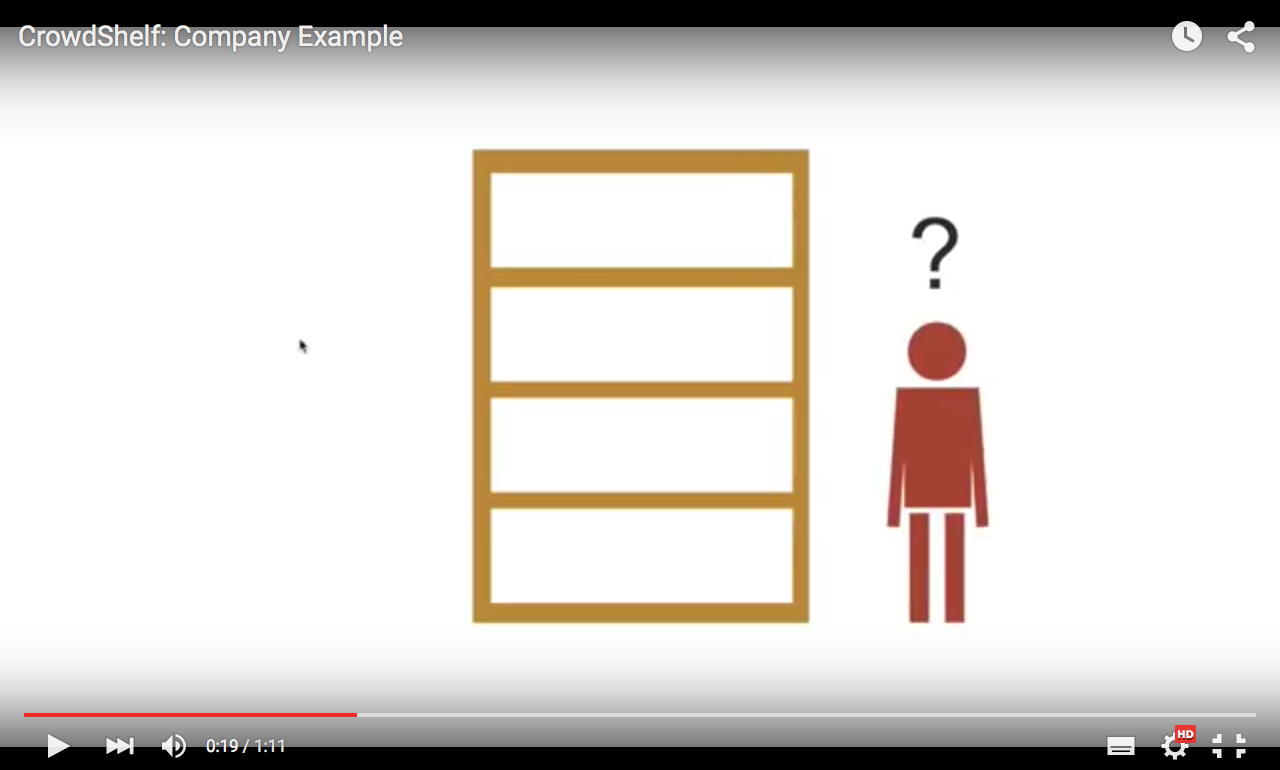
\includegraphics[height=5cm]{figs/v01/InfoMovieCompany1.png}
\caption{Shot from the company example demonstration movie}
\label{fig:company-example}
\end{figure}

\subsubsection{Android}
The Android team encountered a few challenges due to limited experience with the platform, and therefore the development took more time than anticipated. The lack of experience with Android development caused the Android team to spend first iteration learning about the Android platform. During this iteration the team watched videos and read tutorials explaining different aspects of the Android platforms, such as how to use tools such as Android Studio and how to test the applications created on a physical Android device.\cite{android-studios}

By end of the iteration the Android team was able to use the camera of a device as a barcode scanner, and also track usage using a third party tracking service called Mixpanel.\cite{mixpanel}

\subsubsection{iOS}
%A lot more information. Tell how everything was done!
During the first iteration, the iOS team started setting up the project by adding Cocoapods and including all necessary libraries. \cite{cocoapods} These included the networking library Alamofire, the database library Realm, and the barcode scanner library MTBBarcodeScanner. \cite{alamofire}\cite{realm}\cite{mtbbarcodescanner} Alamofire and Realm enables effortless parsing and deserialization of \gls{JSON} responses, and greately reduces the complexity of the interaction with external services.  \cite{json}

The team also did some research to determine the easiest way to distribute and test beta versions of the application. There were many tools available, but only Apple's proprietary TestFlight enabled distribution to external testers without manually registering multiple devices on the Apple Developer Program license. \cite{testflight}\cite{apple-developer-program} Thus TestFlight became the obvious choice.

After the necessary tools were selected, the development of the application could begin. The application would have a data-driven approach, and therefore the first task was to create the data models necessary for the application. \cite{data-driven-programming} These included User, Book, and BookInformation classes. The User contains information such as \gls{ID}, username, email, and name. The Book object contains information from the CrowdShelf backend about the books \gls{ID}, \gls{ISBN}, the owner, who the book is rented to, and whether it is currently available for rent. The book information contains general information about a book retrieved from a third party information provider such as title, authors, and summary. For this version only Google Books \gls{API} was added as an endpoint for information, but the system was designed to easily handle additional endpoints at a later time.\cite{google-books-api}

All user interfaces were designed using the Xcode \gls{IDE}'s built in user interface builder, and were assigned a view controller. For this version, only a simple book view, shelf view and scanner view were implemented.


\subsubsection{Backend}
The first iteration of the \gls{backend} included quite a lot of implementation and code. First of all, the backend team decided on what to build the \gls{backend} with, which was the document-oriented database system MongoDB, and NodeJS with ExpressJS. \cite{mongodb}\cite{node-about}\cite{express} Then the team set up the project, and created a readme-file with installation instructions, and a outline of data model and \gls{API}. This was the only documentation for the \gls{API} for a few versions. The readme-file was shared with  the other development teams, so they knew what they would be working with.

Then the team started coding, by setting up some models for the entities books, users and crowds. These models are modules that present an \gls{API} to other modules to find, update and insert documents into the database. The team also set up a router with the routes, and controllers for the entities. The controllers hold the actual logic surrounding each request. 

The team also set up an environment for which the client applications could use the \gls{API}. This was done with Heroku, together with MongoLab.\cite{heroku}\cite{mongolab} Heroku hosted the server, under the domains \url{http://crowdshelf.herokuapp.com} and \url{http://crowdshelf-dev.herokuapp.com}, while MongoLab held two separte databases for us. The first domain served the code from the \code{master}-\gls{branch} on GithHub, while the second served the code from the development \gls{branch}. For each iteration the team decided to merge the development \gls{branch} into the master \gls{branch}, so that the team had a stable version of the server somewhere, while the team developed new features. Heroku pulled changed from GitHub and restarted the server automatically when something was changed on either branches. This structure is still in place, even though our the main location for the stable version of the server was changed in a later iteration. 

By setting up the server, database and making it available to the development teams working on the client application, the backend team completed its requirements for this iteration.

\subsection{Feedback}
The feedback received from the the initial demonstration movie is mentioned in the planning phase. In other words the vital feedback was collected from the second version of the smoke test where the stories to show use of the application emerged with new clarity. The responses was received through the survey shown in figure \ref{fig:0.1-survey} 

Although the feedback acquired from the survey was positive there were only fifteen responses, which is not sufficient to use as the basis for continued development. Additionally, not all of the responses contained an e-mail address so there was not possible for the team to give the, information about updates. The answers from the survey can be are shown in table \ref{feedback-v1}.

In spite these results, the customer representative stated that the solution conveyed in the videos adequately reflected his needs as a customer. He therefore allowed the development to proceed with the functionality shown in the movies as the concept of the application.

\begin{figure}
\centering
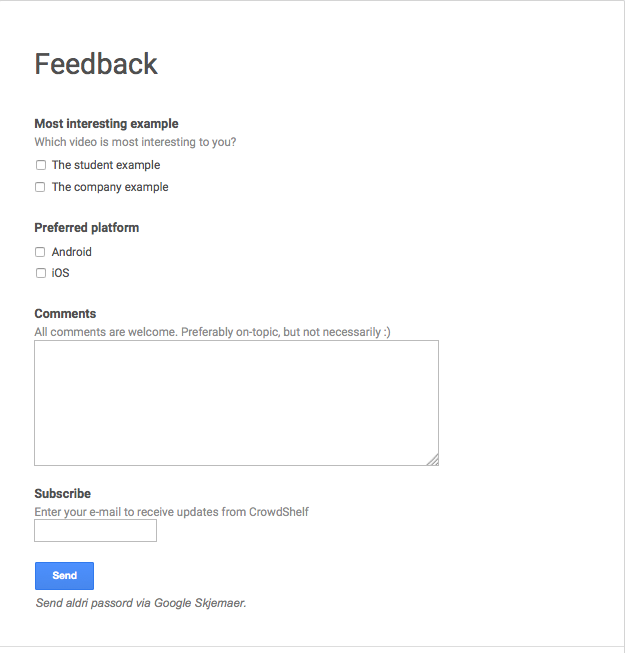
\includegraphics[height=7cm]{figs/v01/01Survey.png}
\caption{The survey from the web page}
\label{fig:0.1-survey}
\end{figure}


\begin{table}[]
\centering
\begin{tabular}{|L{2cm}|L{4.5cm}|L{2cm}|L{2.5cm}|L{3cm}|}
\hline
\textbf{Timestamp} & \textbf{E-mail} & \textbf{Preferred platform} & \textbf{Preferred example} & \textbf{Comments} \\
 \hline

07.09.2015 & jacke.andersson@gmail.com &iOS	  & The company example & - \\
 \hline
 09.09.2015 &  fredsg@gmail.com& Android & The student example  & - \\
 \hline
09.09.2015 & - & Android, iOS  & Both & - \\
 \hline
09.09.2015 & - & Android & The company example & - \\
 \hline
09.09.2015 & - & Android & The student example & Interessting movie! Maybe information about the book standard? \\
 \hline
09.09.2015 &-  & Android & The student example & Nice video, seems like a simple and good app \\
 \hline
09.09.2015 & annakastet@gmail.com & Android & Both & - \\
 \hline
09.09.2015 & peder.kongelf@gmail.com & iOS	 & The company example & More focus on integration with amazon and recommended books \\
 \hline
09.09.2015 &-  & iOS	 & The student example & - \\
 \hline
 10.09.2015 & - & iOS	 & The student example & - \\
 \hline
12.09.2015 & roald40@hotmail.com & Android & The student example & Splendid! Looks very helpful for students as myself. I like it :)  \\
 \hline
20.09.2015 & -& Android & The student example & Top nice app you guys \\
 \hline
05.10.2015 & - & Android & The student example & -\\
 \hline
05.10.2015 & martinwidding@hotmail.com & Android & The company example & Good brand name, cool idea. The Company example is both more appealing, and you do not feel "talked down to" (as in dumbed down) \\
 \hline
16.10.2015 & - & iOS	 & The company example & - \\
 \hline

 
\end{tabular}
\caption{Feedback from survey}
\label{feedback-v1}
\end{table}

\subsection{Version progress}
During this version a lot of tasks were completed to create the foundation of the application. There were administrative tasks that had to be done and new knowledge to be acquired. A figure of the task progression is shown in figure  \ref{fig:progress-v1}.

\begin{figure}
\centering
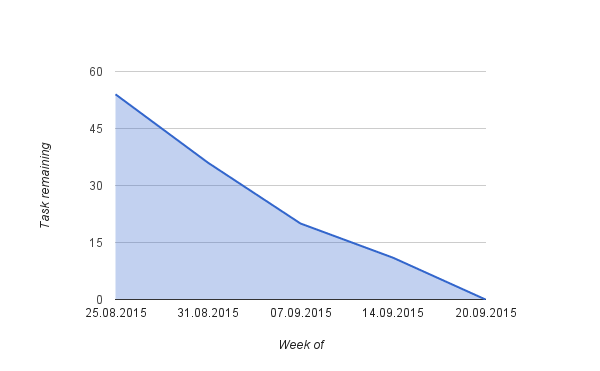
\includegraphics[height=10cm]{figs/v01/progressv1.png}
\caption{Task progression version 0.1}
\label{fig:progress-v1}
\end{figure}


As illustrated in the figure the progress was very good in the first two weeks, while the progress slowed down in the third week. There are two reasons to explain that freeze. The first is that many of the tasks were not in context to implementation which means that the team knew how to complete them. The release note that explains the tasks done in this version is shown in appendix \ref{app:release-note-1}.

As week three was completed the team had encountered some problems which is the other reason. The setback occurred when the implementation had begun and the \gls{API} had to be rewritten to follow rest standard. In addition the Android team learned that they had to remake the structure. 

By the fourth week the project moved forward after the setback by not rushing the implementation and taking the time to learn the different structures of the platforms used for implementation. 

To continuously describe the process to the customer and supervisor the team wrote a blog. The blog posts that were written in this version are shown in figure \ref{fig:week-one}-\ref{fig:week-four}

\newpage
\begin{figure}
\centering
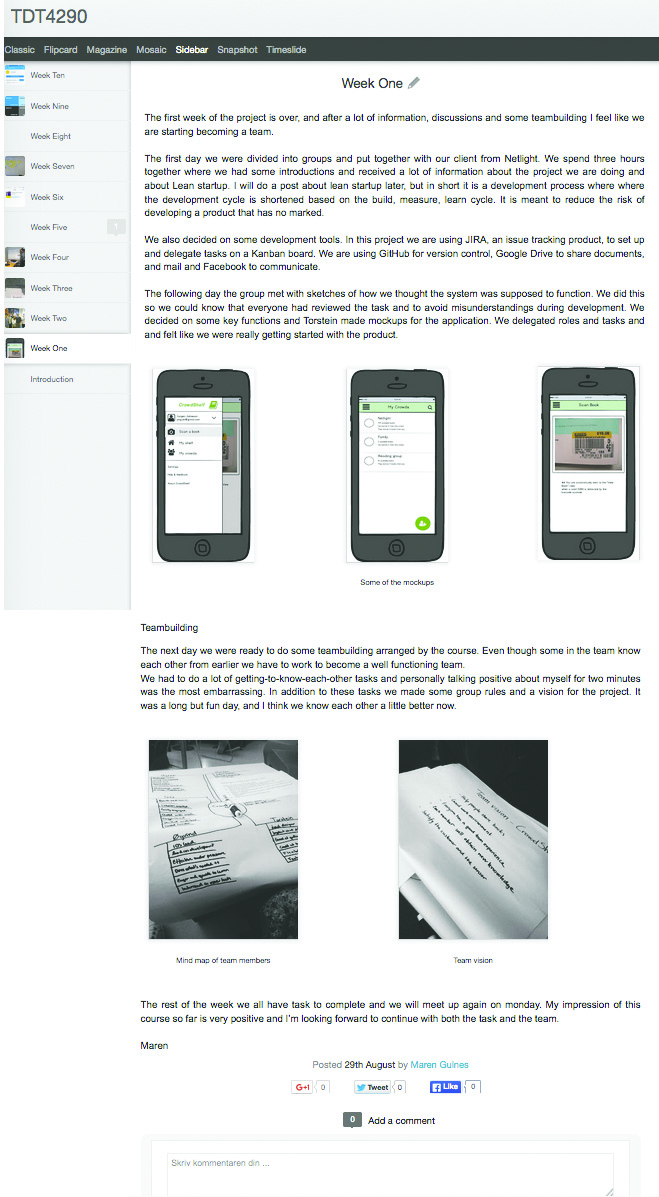
\includegraphics[height=22cm]{figs/v01/WeekOne.jpg}
\caption{Blog post from week 35}
\label{fig:week-one}
\end{figure}

\begin{figure}
\centering
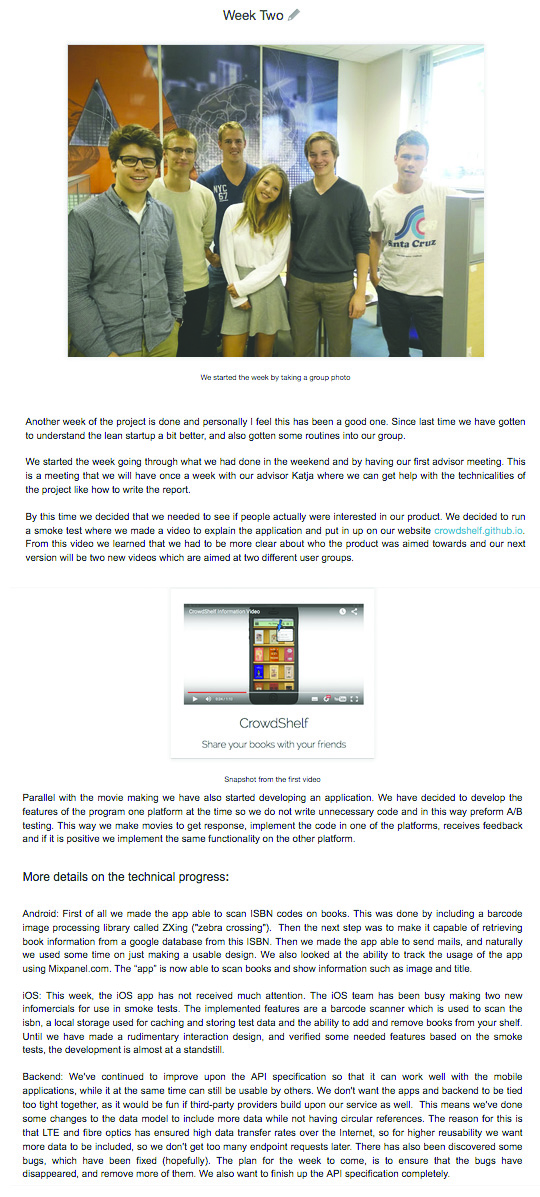
\includegraphics[height=22cm]{figs/v01/WeekTwo.jpg}
\caption{Blog post from week 36}
\label{fig:week-two}
\end{figure}

\begin{figure}
\centering
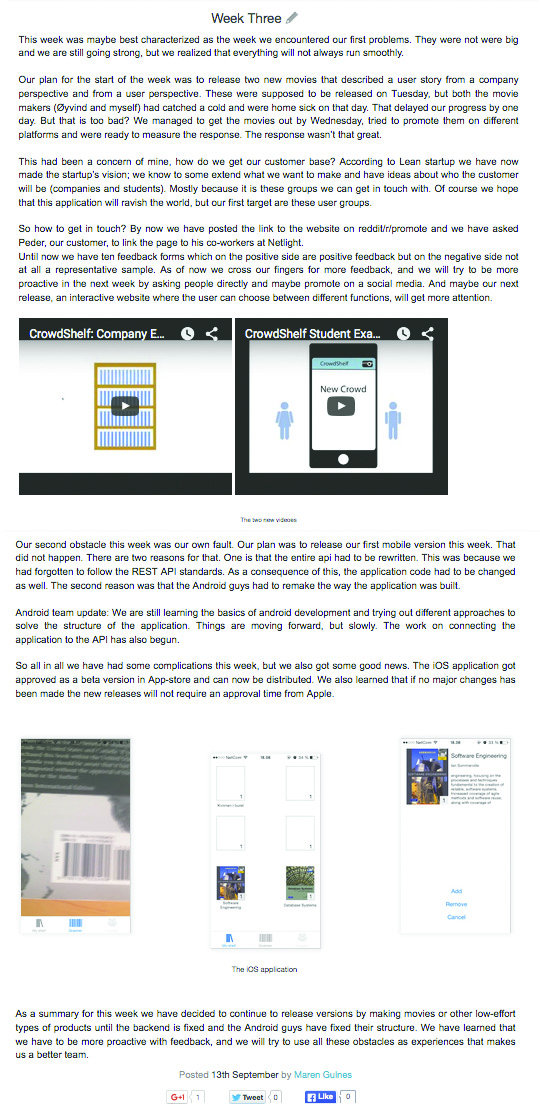
\includegraphics[height=22cm]{figs/v01/WeekThree.jpg}
\caption{Blog post from week 37}
\label{fig:week-three}
\end{figure}

\begin{figure}
\centering
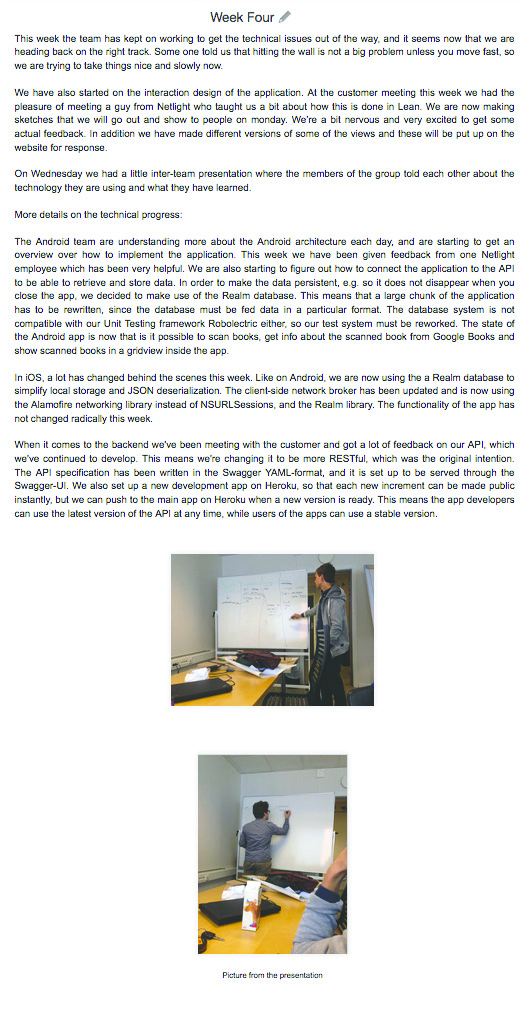
\includegraphics[height=22cm]{figs/v01/WeekFour.jpg}
\caption{Blog post from week 38}
\label{fig:week-four}
\end{figure}

\newpage
\subsection{Review and Retrospective}

In this project the review by the customer happens every week where in a customer meeting where the team presents what is new from the last meeting. The customer contact was very pleased in the beginning of the version with the effort put in the movies and how the team learned about the Lean Startup. He also came with comments on how he wanted the representations in the meetings to be done. From the fourth meeting he requested a demonstration video of the applications each week. It was also he who requested the \gls{API} to follow the REST standards. 

At the end of the version the team had a retrospective meeting where the team members talked about what went well and what could be improved in the iteration. Positive in the version was the interaction in the team. All the team members felt that the communication was good, and that everyone worked the hours they were supposed to. On the less positive side was how the structure of the iteration had been performed. There should be clearer common goals, and more focus on following the Lean Startup.

The three subteams all produced some basic software for the product, and became more familiar with the technologies that were going to be used. There were many lessons to be learned, but by the end of this version the team has achieved a greater understanding of how this project will be structured, and the about the technical issues in their domain.  


\subsection{Summary}
At the beginning of this first version, the team had did not know what the features of the finished product would be. Through a smoke test with videos and surveys, and discussions with the customer representative, the concept for the application has been decided. The team will now focus on deciding what functionality is most important in the application to show how the product will function.

Allowing the to work on their respective tasks for the user stories in parallel with the video proved to be a good decision. It enabled the the clients and server to be synchronized in future iterations.

